%% LyX 2.3.0 created this file.  For more info, see http://www.lyx.org/.
%% Do not edit unless you really know what you are doing.
\documentclass[english]{article}
\usepackage[latin9]{inputenc}
\usepackage{geometry}
\geometry{verbose,tmargin=2cm,bmargin=2cm,lmargin=2cm,rmargin=2cm}
\usepackage{float}
\usepackage{graphicx}

\makeatletter

%%%%%%%%%%%%%%%%%%%%%%%%%%%%%% LyX specific LaTeX commands.
%% Because html converters don't know tabularnewline
\providecommand{\tabularnewline}{\\}

\makeatother

\usepackage{babel}
\begin{document}

\part*{Ejercicio 3}

Se desean realiazar dos modulos en Verilog, un Decoder de dos entradas
y un Mux de cuatro entradas. Ademas de esos dos modulos se implemento
un Encoder.

El programa que se realizo en Verilog, fue hecho con if statments,
esto quiere decir que este, es ajeno a las compuertas logicas y a
su distribucion necesarias para poner en funcionamiento el circuito.
A continuacion, se insertaran figuras de estos tres circuitos, para
poder entender el funcionamiento de estos.

\begin{figure}[H]
\begin{centering}
\includegraphics[scale=0.4]{\string"Untitled Diagram-2\string".png}\caption{Decoder de dos entradas}
\par\end{centering}
\end{figure}

Este es un decoder como el que se realizo en el programa, tiene dos
entradas y cuatro salidas y su tabla de verdad es:
\begin{center}
\begin{tabular}{|c|c|c|c|c|c|}
\hline 
Input 1 & Input 2 & Output 1 & Output 2 & Output 3 & Output 4\tabularnewline
\hline 
\hline 
0 & 0 & \textbf{1} & \textbf{0} & \textbf{0} & \textbf{0}\tabularnewline
\hline 
0 & 1 & \textbf{0} & \textbf{1} & \textbf{0} & \textbf{0}\tabularnewline
\hline 
1 & 0 & \textbf{0} & \textbf{0} & \textbf{1} & \textbf{0}\tabularnewline
\hline 
1 & 1 & \textbf{0} & \textbf{0} & \textbf{0} & \textbf{1}\tabularnewline
\hline 
\end{tabular}
\par\end{center}

\begin{figure}[H]
\begin{centering}
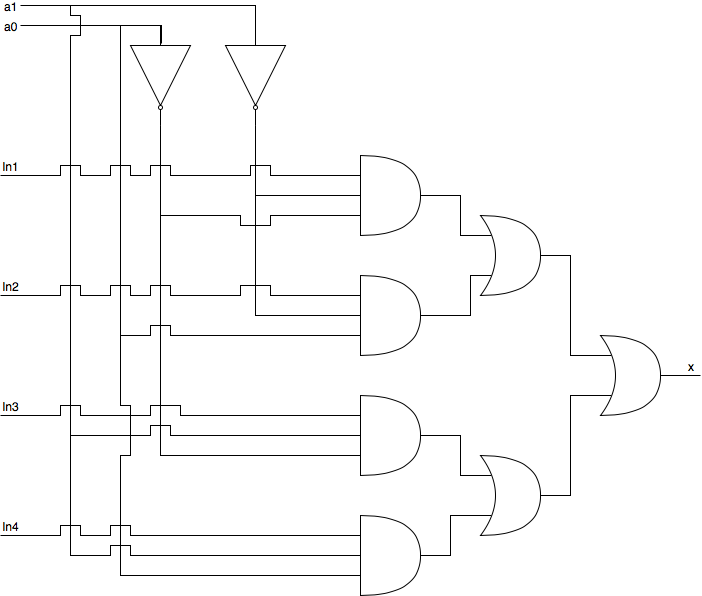
\includegraphics[scale=0.4]{Mux}
\par\end{centering}
\caption{Mux de 4 entradas}

\end{figure}

Este es un Mux como el que se realizo en el progama, tiene cuatro
entradas, una salida y dos select lines. La tabla de verdad es:
\begin{center}
\begin{tabular}{|c|c|c|}
\hline 
a1 & a0 & $x$\tabularnewline
\hline 
\hline 
0 & 0 & \textbf{In1}\tabularnewline
\hline 
0 & 1 & \textbf{In2}\tabularnewline
\hline 
1 & 0 & \textbf{In3}\tabularnewline
\hline 
1 & 1 & \textbf{In4}\tabularnewline
\hline 
\end{tabular}
\par\end{center}

\begin{figure}[H]
\begin{centering}
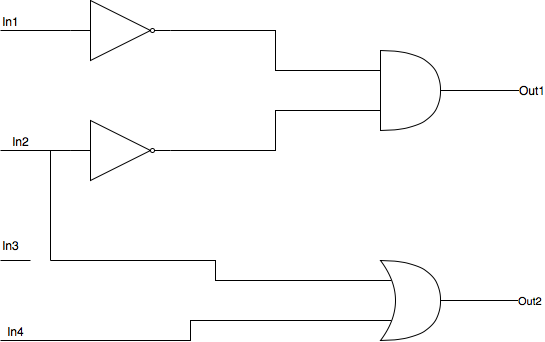
\includegraphics[scale=0.55]{encoder}
\par\end{centering}
\caption{Encoder de 4 entradas}

\end{figure}
Este es un encoder como el que se realizo en Verilog, es de 4 entradas
y dos salidas. La tabla de verdad es:
\begin{center}
\begin{tabular}{|c|c|c|c|c|c|}
\hline 
In1 & In2 & In3 & In4 & Out1 & Out2\tabularnewline
\hline 
\hline 
1 & 0 & 0 & 0 & \textbf{0} & \textbf{0}\tabularnewline
\hline 
0 & 1 & 0 & 0 & \textbf{0} & \textbf{1}\tabularnewline
\hline 
0 & 0 & 1 & 0 & \textbf{1} & \textbf{0}\tabularnewline
\hline 
0 & 0 & 0 & 1 & \textbf{1} & \textbf{1}\tabularnewline
\hline 
\end{tabular}
\par\end{center}

Como se puede ver en la figura 3, una de las entradas no esta conectada
al circuito, pero esto no modifica la salida, ya que puede ser 1 en
un solo caso, en el cual todas las demas entradas son 0, en el resto
de los casos, In3 es siempre 0.
\end{document}
